%! TEX root = introtikz.tex
\documentclass[../geometrymemo.tex]{subfiles}

\begin{document}
\section{Introduction to Ti\textit{k}Z (Ti\textit{k}Z への入門) --- Ti\textit{k}Z の基礎}
\label{sec:introtikz}

In this section, we will try some codes explained here: \url{http://phys.co-suite.jp/tex/Intro_Tikz.pdf}.

\subsection{座標を指定する構文}

\underline{基本}

\begin{lstlisting}[
    language={[LaTeX] TeX},breaklines=true,gobble=4]
    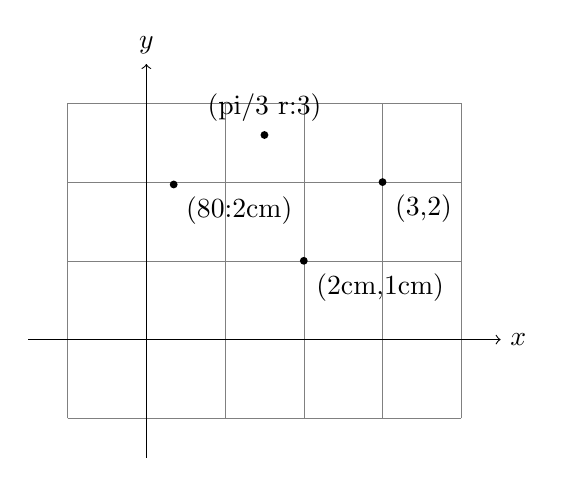
\begin{tikzpicture}[point/.style={fill,shape=circle,inner sep=1pt,outer sep=0pt}]
    \draw[help lines] (-1,-1) grid (4,3);
    % x 軸とy 軸
    \draw[->] (-1.5,0) --(4.5,0) node[right]{$x$};
    \draw[->] (0,-1.5) --(0,3.5) node[above]{$y$};
    % point (値は label で表示）
    \node[point,label=below right:{(2cm,1cm)}] at (2cm,1cm) {};
    \node[point,label=below right:{(80:2cm)}] at (80:2cm) {};
    \node[point,label=below right:{(3,2)}] (C) at (3,2) {};
    \node[point,label=above:{(pi/3 r:3)}] at (pi/3 r:3) {};
    \end{tikzpicture}
\end{lstlisting}
\[
    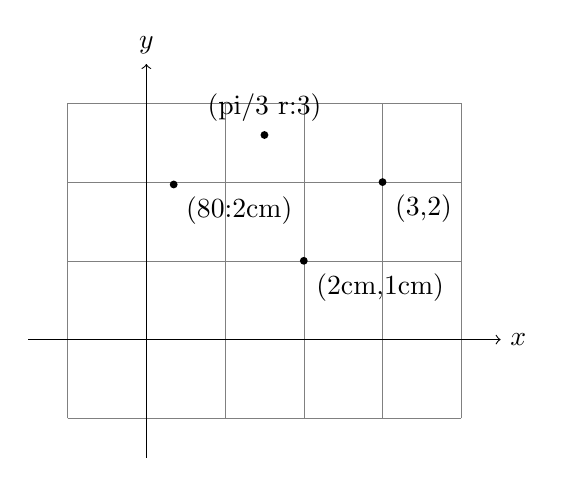
\begin{tikzpicture}[point/.style={fill,shape=circle,inner sep=1pt,outer sep=0pt}]
    \draw[help lines] (-1,-1) grid (4,3);
    % x 軸とy 軸
    \draw[->] (-1.5,0) --(4.5,0) node[right]{$x$};
    \draw[->] (0,-1.5) --(0,3.5) node[above]{$y$};
    % point (値は label で表示）
    \node[point,label=below right:{(2cm,1cm)}] at (2cm,1cm) {};
    \node[point,label=below right:{(80:2cm)}] at (80:2cm) {};
    \node[point,label=below right:{(3,2)}] (C) at (3,2) {};
    \node[point,label=above:{(pi/3 r:3)}] at (pi/3 r:3) {};
    \end{tikzpicture}
\]

\underline{相対位置による座標指定}

\begin{lstlisting}[
    language={[LaTeX] TeX},numbers=none,breaklines=true,gobble=4]
    \begin{tikzpicture}
        \draw (1,0) --++(4,0) --+(1,1) --+(1,-1);
    \end{tikzpicture}
\end{lstlisting}
\[
    \begin{tikzpicture}
        \draw (1,0) --++(4,0) --+(1,1) --+(1,-1);
    \end{tikzpicture}
\]

\subsection{パス path 上のアクション}

\underline{描画のアクション}

\begin{lstlisting}[
    language={[LaTeX] TeX},numbers=none,breaklines=true,gobble=4]
    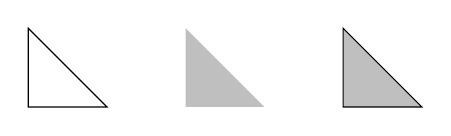
\begin{tikzpicture}[fill=lightgray]
        \path[draw] (1,0) --(0,0) --(0,1) --cycle; % \draw と同じ
        \path[fill,xshift=2cm] (1,0) --(0,0) --(0,1) --cycle; % \fill と同じ
        \path[draw,fill,xshift=4cm] (1,0) --(0,0) --(0,1) --cycle; % \filldraw と同じ
    \end{tikzpicture}
\end{lstlisting}
\[
    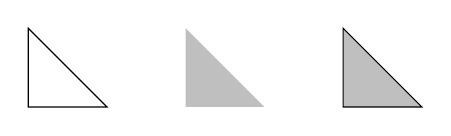
\begin{tikzpicture}[fill=lightgray]
        \path[draw] (1,0) --(0,0) --(0,1) --cycle; % \draw と同じ
        \path[fill,xshift=2cm] (1,0) --(0,0) --(0,1) --cycle; % \fill と同じ
        \path[draw,fill,xshift=4cm] (1,0) --(0,0) --(0,1) --cycle; % \filldraw と同じ
    \end{tikzpicture}
\]

\underline{重なる図形}

\begin{lstlisting}[
    language={[LaTeX] TeX},numbers=none,breaklines=true,gobble=4]
    
\begin{tikzpicture}
        \begin{scope}
            \fill[black] (0,0) rectangle(2,2);
            \fill[lightgray] (1,1) rectangle(3,3);
        \end{scope}
        \begin{scope}[xshift=4cm]
            \fill[lightgray] (1,1) rectangle(3,3);
            \fill[black] (0,0) rectangle(2,2);
        \end{scope}
    \end{tikzpicture}
\end{lstlisting}
\[
    
\begin{tikzpicture}
        \begin{scope}
            \fill[black] (0,0) rectangle(2,2);
            \fill[lightgray] (1,1) rectangle(3,3);
        \end{scope}
        \begin{scope}[xshift=4cm]
            \fill[lightgray] (1,1) rectangle(3,3);
            \fill[black] (0,0) rectangle(2,2);
        \end{scope}
    \end{tikzpicture}
\]

\subsection{図に関するパラメータ}

\underline{オプションの指定}

\begin{lstlisting}[
    language={[LaTeX] TeX},numbers=none,breaklines=true,gobble=4]
    
\begin{tikzpicture}
        \draw[color=gray,fill=lightgray,line width=3pt] (1,0) --(0,0) --(0,1) --cycle;
    \end{tikzpicture}
\end{lstlisting}
\[
    
\begin{tikzpicture}
        \draw[color=gray,fill=lightgray,line width=3pt] (1,0) --(0,0) --(0,1) --cycle;
    \end{tikzpicture}
\]

\subsection{ノード node}

\underline{ノード}

\begin{lstlisting}[
    language={[LaTeX] TeX},numbers=none,breaklines=true,gobble=4]
    \begin{tikzpicture}
    \node[draw] at (0,1) {射};
    \draw[->] (0,0) node[left] {$A$} -- node[above] {$f$} (1,0) node[right] {$B$};
    \draw[help lines,red] (0,1) --(0,0) --(1,0);
    \end{tikzpicture}
\end{lstlisting}
\[
    \begin{tikzpicture}
    \node[draw] at (0,1) {射};
    \draw[->] (0,0) node[left] {$A$} -- node[above] {$f$} (1,0) node[right] {$B$};
    \draw[help lines,red] (0,1) --(0,0) --(1,0);
    \end{tikzpicture}
\]

\underline{ノードの形状}

\begin{lstlisting}[
    language={[LaTeX] TeX},numbers=none,breaklines=true,gobble=4]
    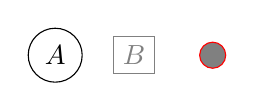
\begin{tikzpicture}
    \draw (0,0) node[draw,circle] {$A$} (1,0) node[draw,rectangle,gray] {$B$} (2,0) node[draw=red,circle,fill=gray] {};
    \end{tikzpicture}
\end{lstlisting}
\[
    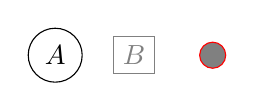
\begin{tikzpicture}
    \draw (0,0) node[draw,circle] {$A$} (1,0) node[draw,rectangle,gray] {$B$} (2,0) node[draw=red,circle,fill=gray] {};
    \end{tikzpicture}
\]

\lstinlineiv{node} の代わりに，\lstinlineiv{coordinate} を指定すれば大きさがゼロのノードを配置できます．ノードに名前を付けることができるため，点にノード名を付けて後で参照できるようにできます．また，\lstinlineiv{label} と組み合わせて使うことが多いです．

図形が重なるときは後に記述した方が上位に来ますが，ノードの場合は１つのパスが最後まで描画された後に配置されます．また，そのノードを使って \lstinlineiv{\draw} するときも，そのノードが上位に来ます．

\underline{ノードと他の図形の重なり}
\begin{lstlisting}[
    language={[LaTeX] TeX},numbers=none,breaklines=true,gobble=4]
    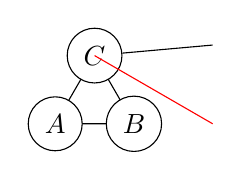
\begin{tikzpicture}[every node/.style={fill=white}]
    \draw (0,0) node[draw,circle] {$A$} --(1,0) node[draw,circle] {$B$} --(60:1) node[draw,circle] (C) {$C$} --cycle;
    \draw (C) --(2,1);
    \draw[red] (C.center) --(2,0);
    \end{tikzpicture}
\end{lstlisting}
\[
    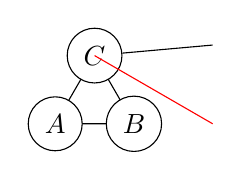
\begin{tikzpicture}[every node/.style={fill=white}]
    \draw (0,0) node[draw,circle] {$A$} --(1,0) node[draw,circle] {$B$} --(60:1) node[draw,circle] (C) {$C$} --cycle;
    \draw (C) --(2,1);
    \draw[red] (C.center) --(2,0);
    \end{tikzpicture}
\]

ノードに名前を付けることができます．そして後からそのノード名を指定することで，ノードを参照することができます．ノード名をつけるには \lstinlineiv{name} オプションを指定するか，\lstinlineiv{node (ノード名)} のように丸カッコでノード名を囲んで指定します．

\underline{ノード名と参照}
\begin{lstlisting}[
    language={[LaTeX] TeX},numbers=none,breaklines=true,gobble=4]
    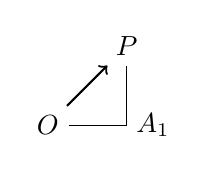
\begin{tikzpicture}
    % ノードへの命名
    \node (O) at (0,0) {$O$};
    \coordinate[{label=right:$A_1$}] (A) at (1,0);
    \node[name=P] at (1,1) {$P$};
    % ノードの参照
    \draw[->,thick] (O) --(P);
    \draw (O) --(A) --(P);
    \end{tikzpicture}
\end{lstlisting}
\[
    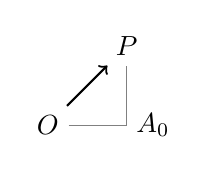
\begin{tikzpicture}
    % ノードへの命名
    \node (O) at (0,0) {$O$};
    \coordinate[{label=right:$A_0$}] (A) at (1,0);
    \node[name=P] at (1,1) {$P$};
    % ノードの参照
    \draw[->,thick] (O) --(P);
    \draw[help lines] (O) --(A) --(P);
    \end{tikzpicture}
\]

\subsection{Using \textbf{\texttt{tcblisting}} BUT NO \textbf{\texttt{minted}}}

First, do NOT use \lstinlineiv{minted}, because it will give warning about \lstinlineiv{fancyvrb}.

To create a side-by-side \LaTeX~source and the typeset output as in 「ノード名と参照1」, use below:
\begin{tcolorbox}
    \begin{verbatim}
\begin{tcblisting}{title=ノード名と参照1,sidebyside,sidebyside gap=1cm,
        righthand width=5cm}
\end{tcblisting}
\end{verbatim}
\end{tcolorbox}
\begin{tcblisting}{title=ノード名と参照1,sidebyside,sidebyside gap=1cm,
        righthand width=5cm}
    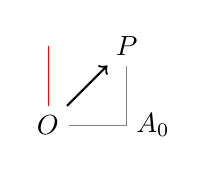
\begin{tikzpicture}
        % ノードへの命名
        \node (O) at (0,0) {$O$};
        \coordinate[{label=right:$A_0$}] (A) at (1,0);
        \node[name=P] at (1,1) {$P$};
        % ノードの参照
        \draw[->,thick] (O) --(P);
        \draw[help lines] (O) --(A) --(P);
        \draw[help lines,red] (O) --(0,1);
    \end{tikzpicture}
\end{tcblisting}

To create a side-by-side, but the typeset output is outside the text as in 「ノード名と参照2」, use below. The point here is \lstinlineiv{listing outside text}.
\begin{tcolorbox}
    \begin{verbatim}
\begin{tcblisting}{title=ノード名と参照2,listing outside text,
        sidebyside,sidebyside gap=1cm,righthand width=5cm}
\end{tcblisting}
\end{verbatim}
\end{tcolorbox}
\begin{tcblisting}{title=ノード名と参照2,listing outside text,
        sidebyside,sidebyside gap=1cm,righthand width=5cm}
    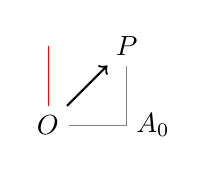
\begin{tikzpicture}
        % ノードへの命名
        \node (O) at (0,0) {$O$};
        \coordinate[{label=right:$A_0$}] (A) at (1,0);
        \node[name=P] at (1,1) {$P$};
        % ノードの参照
        \draw[->,thick] (O) --(P);
        \draw[help lines] (O) --(A) --(P);
        \draw[help lines,red] (O) --(0,1);
    \end{tikzpicture}
\end{tcblisting}

In case the numbered-list is 1-digit only (up to 9 lines of codes), as in 「ノード名と参照3」, then use \lstinlineiv{left=3.8mm}.
\begin{tcolorbox}
    \begin{verbatim}
\begin{tcblisting}{title=ノード名と参照3,left=3.8mm}
\end{tcblisting}
\end{verbatim}
\end{tcolorbox}
\begin{tcblisting}{title=ノード名と参照3,left=3.8mm}
    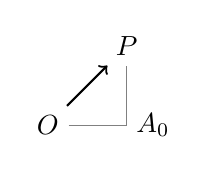
\begin{tikzpicture}
        % ノードへの命名
        \node (O) at (0,0) {$O$};
        \coordinate[{label=right:$A_0$}] (A) at (1,0);
        \node[name=P] at (1,1) {$P$};
        % ノードの参照
        \draw[->,thick] (O) --(P);
        \draw[help lines] (O) --(A) --(P);
    \end{tikzpicture}
\end{tcblisting}

Finally, as shown in 「ノード名と参照4」 when the line number is not needed, set \lstinlineiv{left=2.8mm} and \lstinlineiv{listing options={style=tcbliststyleiv,numbers=none}}. Furthermore, \lstinlineiv{colback=white,enhanced jigsaw} will change the background color to white, and change the skin from the preset \lstinlineiv{bicolor jigsaw} to \lstinlineiv{enhanced jigsaw}, such that the source-typeset-separator-dashed-line will re-appear.
\begin{tcolorbox}
    \begin{verbatim}
\begin{tcblisting}{title=ノード名と参照4,left=2.8mm,
        listing options={style=tcbliststyleiv,numbers=none},
        colback=white,enhanced jigsaw}
\end{tcblisting}
\end{verbatim}
\end{tcolorbox}
\begin{tcblisting}{title=ノード名と参照4,left=2.8mm,
        listing options={style=tcbliststyleiv,numbers=none},
        colback=white,enhanced jigsaw}
    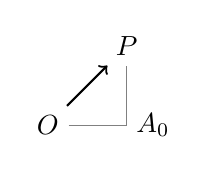
\begin{tikzpicture}
        % ノードへの命名
        \node (O) at (0,0) {$O$};
        \coordinate[{label=right:$A_0$}] (A) at (1,0);
        \node[name=P] at (1,1) {$P$};
        % ノードの参照
        \draw[->,thick] (O) --(P);
        \draw[help lines] (O) --(A) --(P);
    \end{tikzpicture}
\end{tcblisting}

Unlike cnltx-example, in tcblisting \verb|\lstinlineiv{\node}| is still usable, like this: \lstinlineiv{\node}.

Also unlike cnltx-example, in tcblisting \lstinlineiv{\begin{lstlisting}...\end{lstlisting}} % chktex 31
, is also still usable.

\begin{lstlisting}[
    language={[LaTeX] TeX},numbers=none,breaklines=true,gobble=4]
    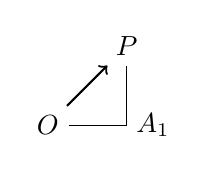
\begin{tikzpicture}
    % ノードへの命名
    \node (O) at (0,0) {$O$};
    \coordinate[{label=right:$A_1$}] (A) at (1,0);
    \node[name=P] at (1,1) {$P$};
    % ノードの参照
    \draw[->,thick] (O) --(P);
    \draw (O) --(A) --(P);
    \end{tikzpicture}
\end{lstlisting}
\[
    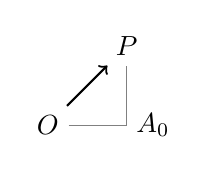
\begin{tikzpicture}
    % ノードへの命名
    \node (O) at (0,0) {$O$};
    \coordinate[{label=right:$A_0$}] (A) at (1,0);
    \node[name=P] at (1,1) {$P$};
    % ノードの参照
    \draw[->,thick] (O) --(P);
    \draw[help lines] (O) --(A) --(P);
    \end{tikzpicture}
\]

\subsection{ツリー，グラフのための構文 Syntax for tree and graph}

１つの \lstinlineiv{node} の後に， \lstinlineiv{child} を続けて記述することでこノードを追加できます．子ノードはいくつも追加できますし，子ノード自身もノードなので，子ノードの子ノードを追加することもできます．
\begin{tcblisting}{title=ツリー構造 (tree structure),sidebyside,sidebyside gap=1cm,
        righthand width=5cm,colback=white}
    \begin{tikzpicture}
        \node {$p$}
        child {node {$q$}
                child {node {$r$}}
                child {node {$s$}
                        child {node {$v$}}
                        child {node {$w$}}
                        child {node {$x$}}
                    }
            }
        child {node {$t$}};
    \end{tikzpicture}
\end{tcblisting}

\lstinlineiv{node} コマンドを使うとノードの配置位置や見た目などを細かく制御できます．しかし，グラフを描くときなど画一的なノードを配置する場合は，graphs ライブラリを使うことでもっと簡潔に記述することができます．
\begin{tcblisting}{title=グラフ (graph),sidebyside,sidebyside gap=1cm,
        righthand width=4cm,colback=white,left=3.8mm}
    % \usetikzlibrary{graphs}
    \begin{tikzpicture} % [every node/.style={draw, circle}]
        \graph[branch right,grow down,nodes={draw,circle}] {
            p[rectangle] -> {q -> {r,s}, t}
        };
    \end{tikzpicture}
\end{tcblisting}

\subsection{オプションパラメータのスコープ (Scope)}

複数のコマンドに対して同じオプションを指定したい場合があります．\lstinlineiv{scope} 環境を使うと，それらで囲まれたコマンドに対して同じオプションを設定できます．
\begin{tcblisting}{title=スコープ (Scope),colback=white,enhanced jigsaw}
    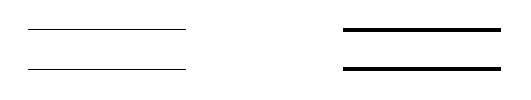
\begin{tikzpicture}
        \begin{scope}[thin]
            \draw (0,0) --(2,0);
            \draw (0,-.5) --(2,-.5);
        \end{scope}
        \begin{scope}[ultra thick,xshift=4cm]
            \draw (0,0) --(2,0);
            \draw (0,-.5) --(2,-.5);
        \end{scope}
    \end{tikzpicture}
\end{tcblisting}

\subsection{スタイル (Style)}

スタイル定義は，\lstinlineiv{スタイル/.style={オプション指定}} の形式で記述します．
\begin{tcblisting}{title=基本,left=3.8mm}
    \begin{tikzpicture}[annot/.style={gray,draw}]
        \node[draw,circle,anchor=south] (p) at (0,0) {$p$};
        \draw[<-] (p) --(2,1) node[annot,right] {ノード $p$};
        \draw[red] (0,0) --(2,1);
    \end{tikzpicture}
\end{tcblisting}

\section{線・図形編}

\subsection{直線を描く}

\begin{tcblisting}{title=\texttt{cycle} を使う場合と使わない場合の違い,left=3.8mm}
    
\begin{tikzpicture}[line width=3mm]
        \draw (0,0) --(1,0) --(1,1) --cycle;
        \draw[xshift=3cm] (0,0) --(1,0) --(1,1) --(0,0);
    \end{tikzpicture}
\end{tcblisting}

\begin{tcblisting}{title=２つの線分を別々に書く場合と連続的に書く場合の違い,left=3.8mm}
    
\begin{tikzpicture}[line width=3mm]
        \draw (0,0) --(1,2); \draw (1,2) --(2,0); % 別々に書く場合
        \draw[xshift=3cm] (0,0) --(1,2) --(2,0); % 連続的に書く場合
    \end{tikzpicture}
\end{tcblisting}

\tcbset{
    colback=white,
    colbacklower=blue!3!white,
    left=3.8mm,
}

\subsection{曲線を描く}

\begin{tcblisting}{title=出射角と入射角を指定する方法}
    \begin{tikzpicture}
        \draw (0,0) to[out=90,in=200](2,1.5); %90度方向へ出射，200度方向から入射
    \end{tikzpicture}
\end{tcblisting}

\begin{tcblisting}{title=曲線を連続的に描画する}
    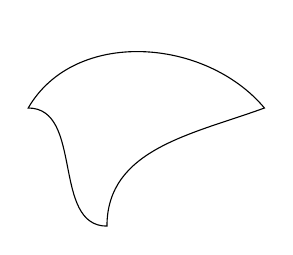
\begin{tikzpicture}
        \draw (0,0) to[out=90,in=200](2,1.5) to[out=130,in=60](-1,1.5) to[out=0,in=180]cycle;
    \end{tikzpicture}
\end{tcblisting}

出射角と入射角にどれだけの速さで近づくかを指定するには \lstinlineiv{looseness} オプションキーを使います．デフォルト値は1です．
\begin{tcblisting}{title=出射角と入射角に近づく速さを指定}
    \begin{tikzpicture}
        \draw (0,0) to[out=0,in=-90,looseness=0.5](1,1);
        \draw[xshift=1.5cm] (0,0) to[out=0,in=-90](1,1);
        \draw[xshift=3cm] (0,0) to[out=0,in=-90,looseness=2](1,1);
    \end{tikzpicture}
\end{tcblisting}

\begin{tcblisting}{title=角度の相対指定}
    
\begin{tikzpicture}
        \draw[very thick] (0,0) to[out=0,in=-90,relative](1,1); % 角度を相対指定
        \draw (0,0) --(1,1);

        \draw[very thick,xshift=1.5cm] (0,0) to[out=0,in=-90](1,1); % 角度を絶対指定
        \draw[xshift=1.5cm] (0,0) --(1,1);
    \end{tikzpicture}
\end{tcblisting}

始点 (0,0) から終点 (1,1) へ向かう直線に対して，\lstinlineiv{bend right} は右に膨らんだ曲線，\lstinlineiv{bend left} は左に膨らんだ曲線になります．また，出射角は指定した相対角度，入射角は \lstinline{180− (指定した相対角度)} になります．次の例 \lstinlineiv{bend right=60} は \lstinlineiv{out=-60,in=240,relative} と同等ということになります．
\begin{tcblisting}{title=角度の相対指定}
    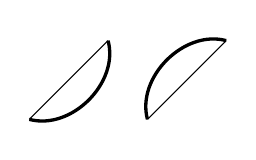
\begin{tikzpicture}
        \draw[very thick] (0,0) to[bend right=60](1,1);
        \draw (0,0) --(1,1);
        \draw[very thick,xshift=1.5cm] (0,0) to[bend left=60](1,1);
        \draw[xshift=1.5cm] (0,0) --(1,1);
    \end{tikzpicture}
\end{tcblisting}

膨らみの量を調整するには，looseness オプションキーの他に distance オプションキーでも指定できます．
\begin{tcblisting}{title=膨らみの量を調整}
    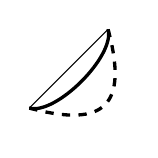
\begin{tikzpicture}
        \draw[very thick] (0,0) to[bend right=60,distance=10pt](1,1);
        \draw[very thick,dashed] (0,0) to[bend right=60,distance=1cm](1,1);
        \draw[thin] (0,0) --(1,1);
    \end{tikzpicture}
\end{tcblisting}

\subsection{矢印を描く}

\begin{tcblisting}{title=連続する線分の矢印 (Draw axes)}
    \begin{tikzpicture}
        \draw[<->] (0,2) |- (2,0);
    \end{tikzpicture}
\end{tcblisting}

矢印のタイプとして，通常の \lstinlineiv{>, >>, >>>, |} や \lstinline{latex, Latex} や \lstinlineiv{stealth, Stealth, Triangle} を使いましょう．
\begin{tcblisting}{title=矢印の基本と倍率でサイズを指定,sidebyside,sidebyside gap=0.4cm,
        righthand width=2.2cm,left=4.6mm}
    \begin{tikzpicture}
        \draw[>->] (0,0) --(2,0);
        \draw[|->] (0,-0.4) --(2.0,-0.4);
        \draw[latex-latex] (0,-0.8) --(2,-0.8);
        \draw[stealth reversed-stealth] (0,-1.2) --(2,-1.2);
        \draw[Stealth-{Stealth[scale=2.5]}] (0,-1.6) --(2,-1.6);
        \draw[latex-{Latex[scale length=2.5]}] (0,-2.0) --(2,-2.0);
        \draw[<-{>[scale width=2pt]}] (0,-2.4) --(2,-2.4);
        \draw[Triangle-{Triangle[orange,length=3mm,width=3mm]}] (0,-2.8) --(2,-2.8);
    \end{tikzpicture}
\end{tcblisting}

\subsection{線の幅を指定する}

\lstinlineiv{line width} または \lstinlineiv{ultra thin, very thin, thin, semithick, thick, very thick, ultra thick} で，デフォルトは， \lstinlineiv{thin} です．

\subsection{線種を指定する}

二重線は double オプションキーを指定することで描画できます．double オプションキーには二重線の間の色を指定できます．デフォルトは white になります．double distance オプションキーには二重線の間隔を指定します．double distance オプションキーを省略すると \qty{0.6}{pt} がデフォルトになります．
\begin{tcblisting}{title=二重線のオプション}
    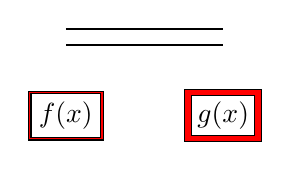
\begin{tikzpicture}
        \draw[double distance=5pt, thick] (0,0) -- (2,0); % 線の間隔を 5pt にする．
        \node[draw, double=red] at (0,-1) {$f(x)$}; % 線の間を red にする．
        \node[draw,double=red,double distance=2pt] at (2,-1) {$g(x)$}; % 線の間を red にする．
    \end{tikzpicture}
\end{tcblisting}

\subsection{長方形を描く}

直線と描くには，２つの座標を \lstinlineiv{to} または \lstinlineiv{--} オペレーションで繋ぎます．同様に，長方形を描くには，２つの座標を \lstinlineiv{rectangle} オペレーションで繋ぎます．
\begin{tcblisting}{title=傾いた長方形}
    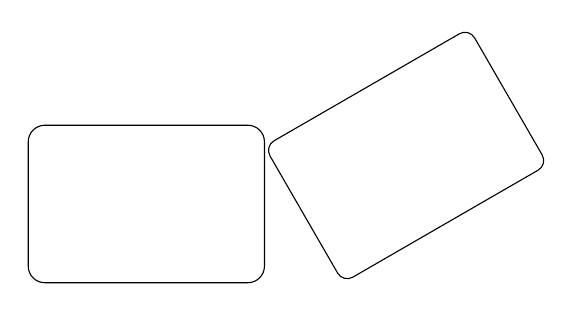
\begin{tikzpicture}
        \draw[rounded corners=6pt] (0,0) rectangle++(3,2);
        \draw[rounded corners,rotate around={30:(4,0)}] (4,0) rectangle++(3,2); % (4,0)を中心に 30度回転した長方形
    \end{tikzpicture}
\end{tcblisting}

\subsection{円・楕円を描く}

\begin{tcblisting}{title=円と傾いた楕円}
    \begin{tikzpicture}
        \draw (0,0) circle[radius=1cm];
        \draw (5,0) circle[x radius=2cm,y radius=1cm,rotate=30];
    \end{tikzpicture}
\end{tcblisting}

\subsection{円弧を描く}

座標として指定するのは円弧の中心ではなく，あくまでも「始点」であることに注意．
\begin{tcblisting}{title=円弧，delta}
    \begin{tikzpicture}
        \draw[red] (0,0) --(4,0);
        \draw[green] (4,0) --(8,0);
        \draw (0,0) arc[radius=1,start angle=45,end angle=270];
        \draw (4,0) arc[x radius=0.5,y radius=1,start angle=45,end angle=270];
        \draw (8,0) arc[radius=1,start angle=45,delta angle=225];
    \end{tikzpicture}
\end{tcblisting}

\subsection{線のつなぎ目をカスタマイズする}

\begin{tcblisting}{title=線のつなぎ目をカスタマイズ}
    \begin{tikzpicture}
        \draw[rounded corners=5mm] (0,0) --(1,0) --(2,1) --(3,1);
        \draw[rounded corners,xshift=4cm] (0,0) --(1,0) --(2,1) --(3,1); % default 4pt
    \end{tikzpicture}
\end{tcblisting}
\begin{tcblisting}{title=パスの途中でつなぎ方を変える}
    \begin{tikzpicture}
        % (1,1) と (2,1) の接続部は丸くつなげる
        \draw (0,0) --(1,0) [rounded corners] --(1,1) --(2,1) [sharp corners] --(2,0) --(3,0);
        \draw[xshift=4cm] (0,0) --(1,0) {[rounded corners] --(1,1) --(2,1)} --(2,0) --(3,0);
    \end{tikzpicture}
\end{tcblisting}
\begin{tcblisting}{title=\texttt{line join} の形状を指定}
    
\begin{tikzpicture}[line width=8pt]
        \draw[line join=miter] (0,0) --(0.5,1.5) --(1,0); % default
        \draw[xshift=3cm,line join=round] (0,0) --(0.5,1.5) --(1,0);
        \draw[xshift=6cm,line join=round] (0,0) --(0.5,1.5) --(1,0) --cycle;
        \draw[xshift=9cm,line join=bevel] (0,0) --(0.5,1.5) --(1,0);
        \draw[xshift=12cm,line join=bevel] (0,0) --(0.5,1.5) --(1,0) --cycle;
    \end{tikzpicture}
\end{tcblisting}

\subsection{交差した線を描く}

\begin{tcblisting}{title=線の交差のさせ方,colbacklower=white}
    
\begin{tikzpicture}[very thick]
        \draw (0,0) --(1,1); % 背面の線
        \draw[line width=6pt,white] (0,1) --(1,0); % 全面の線と同じ線を白い太線で引く
        \draw (0,1) --(1,0);
    \end{tikzpicture}
\end{tcblisting}
\begin{tcblisting}{title=線の交差のさせ方 (\texttt{preaction} 版),colbacklower=white}
    
\begin{tikzpicture}[very thick]
        \draw (0,0) --(1,1); % 背面の線
        \draw[preaction={draw=white,line width=6pt}] (0,1) --(1,0); % 全面の線を引く
    \end{tikzpicture}
\end{tcblisting}

\section{座標編}

\subsection{相対的な座標指定}

\begin{tcblisting}{title=正三角形を \texttt{+} で描く,sidebyside,sidebyside gap=1cm,
        righthand width=5cm}
    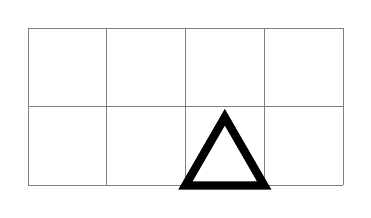
\begin{tikzpicture}[line width=3pt]
        \draw[help lines] (0,0) grid(4,2);
        \draw (2,0) --+(1,0) --+(60:1) --cycle;
    \end{tikzpicture}
\end{tcblisting}

\subsection{関数を使った座標指定}

\begin{tcblisting}{title=星形}
    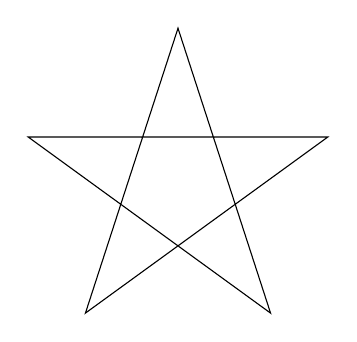
\begin{tikzpicture}
        \foreach \n in {0,1,...,4}
        \coordinate (A\n) at ({2*cos(90+360/5*\n)}, {2*sin(90+360/5*\n)});
        \draw (A0) --(A2) --(A4) --(A1) --(A3) --cycle;
    \end{tikzpicture}
\end{tcblisting}

\subsection{マトリックス状に配置する}

\begin{tcblisting}{title=マトリックス状に配置,left=4.8mm}
    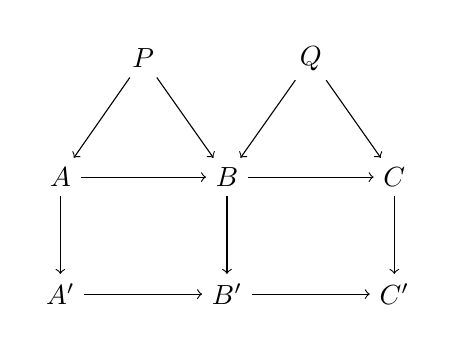
\begin{tikzpicture}
        \matrix[row sep=1cm,column sep=0.5cm] {
                               & \node (P) {$P$}; &                    & \node (Q) {$Q$}; &                    \\
            \node (A) {$A$};   &                  & \node (B) {$B$};   &                  & \node (C) {$C$};   \\
            \node (Ap) {$A'$}; &                  & \node (Bp) {$B'$}; &                  & \node (Cp) {$C'$}; \\
        };
        \draw[->] (P) --(A); \draw[->] (P) --(B);
        \draw[->] (Q) --(B); \draw[->] (Q) --(C);
        \draw[->] (A) --(B); \draw[->] (B) --(C);
        \draw[->] (Ap) --(Bp); \draw[->] (Bp) --(Cp);
        \draw[->] (A) --(Ap); \draw[->] (B) --(Bp); \draw[->] (C) --(Cp);
    \end{tikzpicture}
\end{tcblisting}

\subsection{座標平面にグリッド線を引く}

\begin{tcblisting}{title=グリッド戦の間隔}
    \begin{tikzpicture}
        % \draw[help lines,ultra thick,red] (0,0) grid(3,3);
        \draw[help lines,step=5mm] (0,0) grid(3,3);
    \end{tikzpicture}
\end{tcblisting}

\section{色編}

\subsection{内部を塗りつぶす}

\lstinlineiv{\path[draw=色]} または \lstinlineiv{\draw[色]} または \lstinlineiv{\draw[color=色]} は，外周を「色」で描くことです．デフォルトの色は黒です．
\begin{tcblisting}{title=外周も描く}
    \begin{tikzpicture}[line width=6pt]
        \draw[gray,fill=red] (0,0) rectangle+(2,1); % 赤で塗りつぶし，グレーで外周を描く．
        \draw[fill=red,xshift=4cm] (0,0) rectangle+(2,1); % 赤で塗りつぶし，デフォルト色で外周を描く．
        \draw[color=blue,fill=red,xshift=8cm] (0,0) rectangle+(2,1);
        \fill[red,xshift=12cm] (0,0) rectangle+(2,1); % 赤で塗りつぶすだけ，外周を描かない．
        \draw[help lines,green] (0,0) --(12,0);
    \end{tikzpicture}
\end{tcblisting}

\begin{tcblisting}{title=閉じていないパスや交差するパスに対する塗りぶつし}
    \begin{tikzpicture}[line width=6pt]
        \draw[fill=red] (0,0) --(0,1) --(2,1) --(2,0); % 閉じていないパス
        \draw[fill=red,xshift=4cm] (0,0) --(0,1) --(2,0) --(2,1); % 閉じていない，かつ交差するパス
        \draw[fill=red,xshift=8cm,line join=round] (0,0) --(0,1) --(2,0) --(2,1) --cycle; % 閉・交差
    \end{tikzpicture}
\end{tcblisting}

\begin{tcblisting}{title=透明度の指定}
    \begin{tikzpicture}
        \draw[fill=red] (0,1) rectangle+(7,1); % 背面の長方形
        \draw[fill=black] (1,0) rectangle+(1,3); % 全面の長方形 opacity=1
        \draw[fill,opacity=0.5] (3,0) rectangle+(1,3); % 全面の長方形 opacity=0.5
        \draw[fill,opacity=0.3] (5,0) rectangle+(1,3); % 全面の長方形 opacity=0.3
    \end{tikzpicture}
\end{tcblisting}

\subsection{図形の一部を塗りつぶす}

\begin{tcblisting}{title=集合の共通部分}
    \begin{tikzpicture}
        \draw (0,0) circle[radius=1]; % A
        \draw (1,0) circle[radius=1]; % B
        \begin{scope}
            \clip (1,0) circle[radius=1]; % Bの形でクリッピングする
            \fill[yellow] (0,0) circle[radius=1]; % スコープの中で A を塗りつぶす
        \end{scope}
    \end{tikzpicture}
\end{tcblisting}

\subsection{ノードの色}

\begin{tcblisting}{title=ノードの色}
    \begin{tikzpicture}
        \node[color=red] at (0,0) {$O$}; % draw しない，つまり外周を描かない．[red] と同じ効果
        \node[draw,red] at (1,0) {$A$}; % foreground色を指定
        \node[draw=blue,text=red] at (2,0) {$B$}; % text 色を指定
        \node[draw=teal,text=red,fill=yellow] at (3,0) {$C$}; % 塗りつぶし色を指定
    \end{tikzpicture}
\end{tcblisting}

\subsection{図全体に背景色をつける}

\begin{tcblisting}{title=Background (背景)色をつける}
    % \usetikzlibrary{backgrounds}
    \begin{tikzpicture}[background rectangle/.style={fill=lightgray,draw=red},
            show background rectangle] % draw をつけない場合，枠線が描画されない
        \fill[gray] (0,0) circle[x radius=2,y radius=1];
    \end{tikzpicture}
\end{tcblisting}
\begin{tcblisting}{title=背景色を \texttt{\{fill=色\}} のように指定しない場合，枠線だけが描画される}
    \begin{tikzpicture}[show background rectangle]
        \fill[gray] (0,0) circle[x radius=2,y radius=1];
    \end{tikzpicture}
\end{tcblisting}

\section{ノード・ラベル編}

\subsection{ノードを配置する}

\begin{tcblisting}{title=ノードの基本}
    \begin{tikzpicture}
        \draw[help lines] (0,0) grid(2,1);
        \node[fill=gray] at (0,0) {}; % ノードのみを配置
        \node[fill=gray] at (1,0) {$A_0$}; % ラベルを持つノード
        \node[fill=gray,label=below:$B_1$] (B1) at (2,0) {}; % Use coordinate for location, NOT node
        \draw[green] (B1) --(1,1); % 参照．ノードは一番上に描画される．
    \end{tikzpicture}
\end{tcblisting}

複数のノードを一つのコマンド列で書けます．また，次の例のように，\textcolor{red}{\textbf{座標指定の後に}} \lstinlineiv{node} オペレーションを記述すると，その座標の位置にノードを配置します．またまた，同じ例に，\textcolor{red}{\textbf{座標指定の前に}} \lstinlineiv{node} オペレーションを記述すると，線分や曲線の途中にラベルを配置することになります．
\begin{tcblisting}{title=複数ノード，座標指定の後か前に \texttt{node} オペレーションを記述する場合の違い}
    \begin{tikzpicture}
        \draw (0,0) --(2,0) node {$A$} --(4,0) node {$B$}; % 線分を引くと同時にラベルを配置
        \draw (0,-1) (2,-1) node {$A'$} (4,-1) node {$B'$}; % 座標指定の後に node を呼ぶ
        \draw (0,-2) --node {$C$} (2,-2) --node {$D$} (4,-2); % 座標指定の前に node を呼ぶ
        \draw (0,-3) to[bend left=30] node {$C'$} (2,-3) to[bend right=30] node {$D'$} (4,-3);
    \end{tikzpicture}
\end{tcblisting}

\begin{tcblisting}{title=相対位置を指定}
    \begin{tikzpicture}
        \draw (0,0) --node[pos=0.1] {$A$} (5,0); % 左から 0.1:0.9 の位置に配置
        \draw (0,-1) --node[midway] {$B$} (5,-1); % 中間の位置に配置
    \end{tikzpicture}
\end{tcblisting}

\subsection{ノードへの命名}

\begin{tcblisting}{title=ノードの命名と参照}
    \begin{tikzpicture}
        \node (A) at (0,0) {$A$};
        \draw (2,0) --node[below] (B) {$B$} (4,0) --(6,0) node[below] (C) {$C$}; % B in the midway!
        \draw (B.north) to[bend left=30] (C.north);
        \draw[very thick,green] (B) --(C);
        \draw[red] (3,0) to[bend right=20] (6,0);
    \end{tikzpicture}
\end{tcblisting}

\subsection{オプションによるノードの位置指定}

\subsubsection{座標や位置を変数にするには，\texttt{coordinate} を使う (VERY IMPORTANT)}

\begin{tcblisting}{title=\texttt{coordinate}'s label default position is above the reference point}
    \begin{tikzpicture}[point/.style={fill,shape=circle,inner sep=3pt,outer sep=0pt}]
        \path coordinate[label=above:$O$] (O) at (0,0) coordinate[label=$A$] (A) at (3,0);
        \coordinate[label=$B$] (B) at (1,1); % \coordinate for single coordinate!
        \path node[point] at (O) {} node[point] at (A) {}; % \path node node, for multi nodes!
        \node[point] at (B) {}; % \node for single node!
        \draw[red,thick] (O) --(A) --(B) --cycle;
        \draw[green] (0,0) to[bend right=30](3,0) to[bend right=30](1,1) to[bend right=30]cycle;
    \end{tikzpicture}
\end{tcblisting}

The above code can be written without \lstinlineiv{at}. Default \lstinlineiv{label distance} is \lstinlineiv{0pt}.
\begin{tcblisting}{title=Use \texttt{coordinate} with \texttt{label} to define coordinate}
    \begin{tikzpicture}[point/.style={fill,shape=circle,inner sep=1pt,outer sep=0pt},label distance=1pt]
        \path (0,0) coordinate[label=left:$O$] (O) (3,0) coordinate[label=right:$A$] (A) (1,1) coordinate[label=$B$] (B); % draw the label
        \draw[red,thick] (O) --(A) --(B) --cycle;
        \draw[green] (0,0) to[bend right=30](3,0) to[bend right=30](1,1) to[bend right=30]cycle;
        \path (O) node[point] {} (A) node[point] {} (B) node[point] {}; % draw points WITHOUT text
    \end{tikzpicture}
\end{tcblisting}

\subsubsection{パスの途中のノード配置}

通常は \lstinlineiv{tikzpicture} 環境に \lstinlineiv{auto} オプションキーを指定します．
\begin{tcblisting}{title=パスの途中のノード (auto option)}
    \begin{tikzpicture}[auto] % auto でノードのテキストが線の上から離す
        \node (A) at (0,2) {$A$}; \node (B) at (2,2) {$B$};
        \node (C) at (0,0) {$C$}; \node (D) at (2,0) {$D$};
        \draw[->] (A) -- node {$f$} (B);% 右向き矢印
        \draw[->] (A) -- node {$g$} (C);% 下向き矢印
        \draw[->, swap] (C) -- node {$p$} (D);% 右向き矢印
        \draw[->, swap] (B) -- node {$q$} (D);% 下向き矢印
    \end{tikzpicture}
\end{tcblisting}
\begin{tcblisting}{title=曲線に沿うラベル}
    \begin{tikzpicture}
        \draw (0,0) to[out=0,in=270] node[above,sloped,near start] {start} node[below,sloped,near end] {end} (5,2); % 曲線上のラベル
    \end{tikzpicture}
\end{tcblisting}

\subsection{ノードの形状，大きさ}

ノードは形状と大きさを持ちます．例えば \lstinlineiv{node} のオプションとして \lstinlineiv{draw} オプションキーを指定すると，\textcolor{red}{\textbf{ノードの形状と大きさにしたがい輪郭が描画されます}}．

\subsubsection{ノードの形状}

\begin{tcblisting}{title=ノードの形状を指定し，輪郭を描画する}
    \begin{tikzpicture}
        \node[draw,rectangle] at (0,0) {ノード};
        \path (3,0) node[draw,circle] {ノード} (6,0) node[draw] {ノード}; % multiple definition
        \node[draw,rounded corners=10pt,inner sep=10pt] at (9,0) {ノード};
    \end{tikzpicture}
\end{tcblisting}
上の例では \verb|draw| オプションキーを \verb|node| に指定しているので，それぞれのノードの形状に沿った輪郭が描画されています．

実は \verb|coordinate| シェイプというのもありますが，これは \lstinlineiv{\coordinate} コマンドによるノード定義と同様，大きさの無いノードにすぎません．\lstinlineiv{coordinate} シェイプは「大きさがない」という形状を意味するシェイプです．

\subsubsection{ノードの輪郭とテキストとの間隔}

ノードの輪郭とテキストの間隔を制御することができます．\lstinlineiv{node} のオプションキーとして \lstinlineiv{inner sep, inner xsep, inner ysep} を指定します．
\begin{tcblisting}{title=輪郭とテキストの間隔}
    \begin{tikzpicture}
        \node[draw,inner sep=10pt] at (0,0) {ノード}; % 上下左右を広げる
        \node[draw,inner xsep=20pt] at (3,0) {ノード}; % 左右を広げる
        \node[draw,inner ysep=20pt] at (6,0) {ノード}; % 上下を広げる
    \end{tikzpicture}
\end{tcblisting}

一方，輪郭とその外との間隔を制御することもできます．\lstinlineiv{node} のオプションキーとして \lstinlineiv{outer sep, outer xsep, outer ysep} を指定します．
\begin{tcblisting}{title=輪郭とその外との間隔}
    \begin{tikzpicture}
        \node[draw,circle,outer sep=5pt] (A) at (0,0) {ノード}; % 上下左右の間隔を空ける
        \node[draw,circle,outer xsep=10pt] (B) at (3,0) {ノード}; % 左右の間隔を空ける
        \node[draw,circle,outer ysep=20pt] (C) at (0,-3) {ノード}; % 上下の間隔を空ける
        \draw (B) --(A) --(C); % 線で結んでみる
    \end{tikzpicture}
\end{tcblisting}

\subsubsection{ノードの大きさをそろえる}

ノードの大きさは中のテキストに合わせて自動的に設定されます．\textcolor{red}{\textbf{ところでノードをいくつか並べた時に，それらのサイズをそろえたいということがあります．}}その場合は，ノードのサイズの最小値を設定することで，それより小さいサイズのテキストであってもノードの大きさを確保することができます．
\begin{tcblisting}{title=ノードのサイズの最小値}
    \begin{tikzpicture}
        \node[draw,minimum size=50pt] (A) at (0,0) {\footnotesize{ノード A}}; % 幅と高さの最小値
        \node[draw,minimum height=50pt] (B) at (3,0) {\large{ノード B}}; % 高さの最小値
        \node[draw,minimum width=50pt] (C) at (0,-2) {ノード C}; % 幅の左右の最小値
    \end{tikzpicture}
\end{tcblisting}

ノードのサイズをそろえるためには各ノードに同じ最小値を設定する必要があります．ですので，通常はスタイルとして設定します．
\begin{tcblisting}{title=ノードのサイズの最小値（スタイル設定）}
    \begin{tikzpicture}[box/.style={minimum size=50pt}]
        \node[draw,box] (A) at (0,0) {\footnotesize{ノード A}};
        \node[draw,box] (B) at (3,0) {\large{ノード B}};
        \node[draw,box] (C) at (0,-2) {ノード C};
    \end{tikzpicture}
\end{tcblisting}

\subsection{オプション指定によるラベル配置}

ラベルもノードの一種です．ノードを配置し，そこにテキストを表示するという考え方がラベル配置の基本になります．ところで，あるノードの隣にラベルを配置するという場合は，オプションを使って簡単にラベルを配置することもできます．

\lstinlineiv{label} オプションキーを \lstinlineiv{label=角度:テキスト} の形式で記述すると，テキストと表示位置の両方を同時に指定できます．\textcolor{red}{\textbf{label オプションキーで配置したラベルも１つのノードであることに注意してください}}．
\begin{tcblisting}{title=\texttt{label} の基本}
    \begin{tikzpicture}
        \node[draw] at (0,0) [label=right:B]{A};
        \node[red,draw,label={[red] right:B}] at (4,0) {A}; % Identical with above but in red
    \end{tikzpicture}
\end{tcblisting}

角度には数値のほか，\lstinlineiv{north} や \lstinlineiv{below left} などが使えます．省略すると \lstinlineiv{above} が指定されます．また，\lstinlineiv{label} のテキストに「カッコ，コンマ，セミコロンなどの特殊文字」を含める場合は，引数全体を波カッコ (curly brace) で囲む必要があります．
\begin{tcblisting}{title=ラベル位置の指定}
    \begin{tikzpicture}
        \node[draw] at (0,0) [label=70.5:a] {\Huge A};
        \node[draw,label=above:b] at (2,0) {\Huge B};
        \node[draw] at (4,0) [label=below left:c] {\Huge C};
        \node[draw] at (6,0) [label=north:d] {\Huge D};
        \node[draw] at (8,0) [label=center:e] {\Huge E};
        \node[draw] at (10,0) [label={above:(1,3);}] {\Huge F}; % カッコ，コンマ，セミコロンを含む
    \end{tikzpicture}
\end{tcblisting}

\lstinlineiv{label} のテキストにオプションを指定することができます．
\begin{tcblisting}{title=\texttt{label} のテキストのオプション}
    \begin{tikzpicture}
        \node[draw] at (0,0) [label={[red,draw,circle,inner sep=8pt] above:{\Huge a}}] {A};
    \end{tikzpicture}
\end{tcblisting}

\lstinlineiv{label} オプションキーを複数指定することで，ラベルを複数配置できます．また，\lstinlineiv{label distance} オプションキーでラベルとノードとの距離を指定できます．
\begin{tcblisting}{title=ラベルの複数配置と距離の指定}
    \begin{tikzpicture}[label distance=5mm]
        \node[draw,circle] at (0,0)
        [label=north:北, label=east:東, label=west:西, label=south:南]
        {\Huge $+$};
    \end{tikzpicture}
\end{tcblisting}

\lstinlineiv{label} オプションキーで配置したラベルもやはりノードの一つですので，ノード名をつけることができます．\lstinlineiv{name} オプションキーを使うことで命名できます．
\begin{tcblisting}{title=\texttt{label} というノードに命名}
    \begin{tikzpicture}[label distance=5mm]
        \node[draw,circle] at (0,0)
        [label={[name=kita] north:北}, label={[name=higashi] east:東},
            label={[name=nishi] west:西}, label={[name=minami] south:南}]
        {\Huge $+$};
        \draw[thick] (kita) --(nishi) --(minami) --(higashi) --(kita);
    \end{tikzpicture}
\end{tcblisting}

ノードとラベルとの間を線で結ぶときは \lstinlineiv{label} オプションキーの代わりに \lstinlineiv{pin} オプションキーを指定します．また，\lstinlineiv{label distance} ではなく，\lstinlineiv{pin distance} を指定します．
\begin{tcblisting}{title=\texttt{pin} でノードからラベルへ線を引く}
    \begin{tikzpicture}[pin distance=10mm]
        \node[draw,circle] at (0,0)
        [pin=north:北, pin=east:東, pin=west:西, pin=south:南]
        {\Huge $+$};
    \end{tikzpicture}
\end{tcblisting}

\lstinlineiv{quotes}ライブラリを使えばラベルの配置がもっと関係にできます．事前に \lstinlineiv{quotes} ライブラリを読み込む必要があります．
\begin{tcblisting}{title=ラベルを \texttt{quotes} で簡潔に配置}
    \begin{tikzpicture}
        % \usetikzlibrary{quotes}
        \node[label=below:A,draw] at (2,0) {B}; % draw option is to draw node B's rectangle
        \node["A" below,draw] at (0,0) {B}; % same meaning as above
        \node[label={[red,circle,draw] below:C},draw] at (0,-1.5) {D};
        \node["C" {below,red,circle,draw},draw] at (2,-1.5) {D}; % same meaning as above
    \end{tikzpicture}
\end{tcblisting}

\subsection{ラベルの複数行表示}

See \url{http://phys.co-suite.jp/tex/Intro_Tikz.pdf} Section 5.8.

\subsection{線上に白抜きのラベルを配置する}

例えば寸法を表示するときに，２点間を直線で結び，その途中に数値を表示したい場合があります．このとき戦を途中で切る必要はありません．単にノードに少し大きさを持たせ，背景色を指定すれば良いです．See also ``how to annotate line with its length''.
\begin{tcblisting}{title=寸法の表示}
    \begin{tikzpicture}
        \coordinate (A) at (0,0);\draw[fill] (A) circle[radius=1pt];
        \coordinate (B) at (2,0);\draw[fill] (B) circle[radius=1pt];
        \draw (A) ++(0,-0.1) -- ++(0,-0.1) coordinate (A1) -- ++(0,-0.1);
        \draw (B) ++(0,-0.1) -- ++(0,-0.1) coordinate (B1) -- ++(0,-0.1);
        \draw[<->] (A1) -- node[inner sep=2mm, fill=white] {\qty{2}{cm}} (B1);
        \draw[help lines] (A) to[bend left=40] node[black,fill=white,midway,inner sep=2.5pt] {\qty{2}{cm}} (B);
        % help lines is thin (normal size), gray color
    \end{tikzpicture}
\end{tcblisting}

\end{document}
